
\section{Service-Oriented Workflows}\label{sec:serviceOrientedWorkflows}

We introduce our approach with a prototypical Friend Finder application, although our approach can be applied to a broader range of applications. Consider a scenario in which multiple users are in an urban area carrying GPS-enabled mobile devices that periodically transmit their location; furthermore, they have agreed to share some of their personal information. A user in this scenario may want to \textit{Find friends which are no more than 3 km away from her, which are over 21 years old and that are interested in art}.
		
Data services produce data in one of two ways: on-demand in response to a given request, or continuously as a data stream. In either case, the data service exposes an interface, composed of several operations and supported by standardized protocols. The JavaScript Object Notation\footnote{JSON http://www.json.org/} is used to represent the data. Accordingly, objects are built from atomic values, nested tuples, and lists.
	
For instance, in our scenario the users' location is available by a stream data service with the interface
	
$\mathtt{subscribe() \rightarrow \lceil location:\langle nickname, coor\rangle\rceil}$
	
consisting of a subscription operation that after invocation will produce a stream of location tuples, each with a nickname that identifies the user and his/her coordinates. The rest of the data is produced by the next two on-demand data services, each represented by a single operation
	
$\mathtt{profile(nickname) \rightarrow person:\langle age, gender, email\rangle}$
\\
$\mathtt{interests(nickname) \rightarrow \left[s\_tag:\langle tag, score\rangle\right]}$
	
	
The first provides a single person tuple denoting a profile of the user, once given a request represented by his/her nickname. The second produces, given the nickname as well, a list of s\_tag tuples denoting the interests of the user by scored tags (\eg{} 'music' with 8.5).
	
In order to obtain the desired result we need to give to it an executable form, in our case a workflow of activities implementing a service coordination. Workflows are built by the parallel and sequential composition of activities that are bound to data and computation services; the first provide the data, while the latter process them as required.

\subsection{Workflow Model}\label{subsec:workflowModel}

The workflow is specified textually as an Abstract State Machine (ASM) \cite{Gurevich1995}, which can be represented as a series-parallel graph. Such representation of a service coordination corresponding to our example application is given in Figure \ref{fig:servCoorExample}. It includes the location, profile, and interests data services, as well as computation services for various relational operations such as selections, joins, and a window bounding the location stream.
		
\begin{figure}
	\centering
		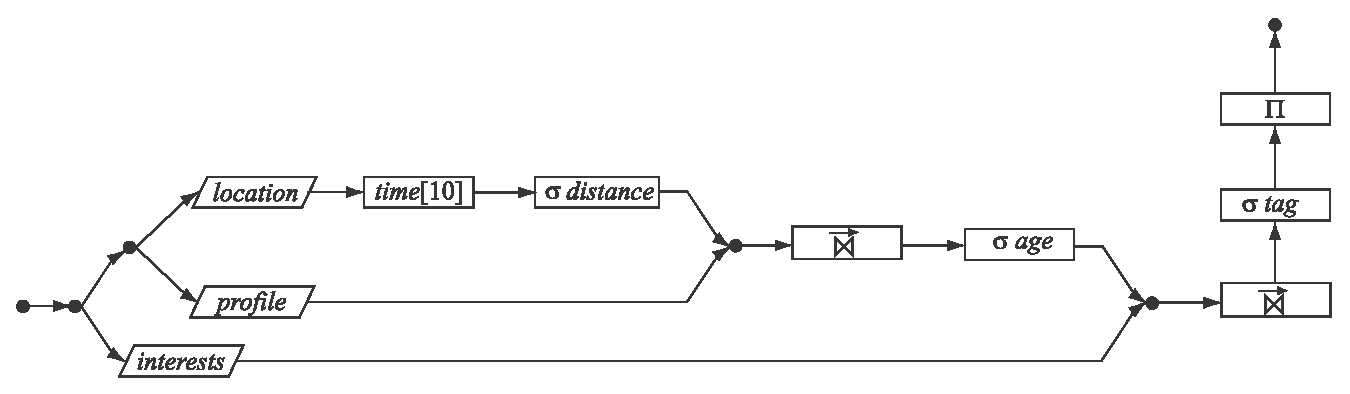
\epsfig{file=Images/FriendFinderQueryWF.eps, scale=0.37}
		\caption{Service-oriented workflow example}
		\label{fig:servCoorExample}
\end{figure}

Concretely, a service-oriented workflow $W$ is modeled as a directed acyclic graph \textit{W=(V, E, init, finish, A, O)} where:
		\begin{center}
			\footnotesize
			\begin{tabular}{rp{5.5cm}}
				$V$                      & is a set of vertices \\
				$E \subseteq V \times V$ & is a set of edges \\
				$A \subseteq V$          & is a set of activities \\
				$\{init, finish\} \subseteq A$     & are the initial and final activities of $W$\\
				$O \subseteq V$          & is a set of workflow composition operators $\{seq_1,...,seq_m,par_1,...,par_n\}$\\.     
			\end{tabular}   
		\end{center}
There are three types of vertices: \textit{activities} perform a service method invocation and always have ancestor and descendant vertices, \textit{init} vertices have no ancestors and their only goal is to launch the first \textit{activity} of the workflow, \textit{finish} vertices have no descendants and stops the workflow execution after the last \textit{activity}.

\subsection{Computation services}\label{subsec:computationServices}

Two kinds of computation services form part of our approach: simple computation services and composite computation services specified in the ASASEL language.
	
\textbf{Simple computation services} These involve a single service operation invocation to process data (see Figure \ref{fig:simpleService}). The distance computation service relies on a \texttt{geo-distance} service, which provides the capability to calculate the geographical distance between two points, e.g., by Vincenty's formula.

\textbf{Composite computation services} These process data by multiple operation invocations, possibly from different services, and often also by the manipulation of local data. These tasks are organized in a service coordination specified in the ASASEL language and represented as a workflow, following a model in which we add data items as well as conditional and iteration constructs to our basic parallel and sequential composition workflow model illustrated in Figure \ref{fig:servCoorExample}.
		
Figure \ref{fig:compositeService} depicts a composite computation service, it evaluates the join operator based on the symmetric hash-join algorithm and two instances of a stateful \texttt{hash-index} service. Several interrelated operation invocations on both service instances, as well as reads and updates on local data items, are used to find the tuple matches that form part of the join result. The specification of a tuple-based window service in ASASEL is presented in Listing \ref{TimeWindowListing}.
		
\begin{figure*}
	\centering
		\begin{tabular}{lr}
				\subfloat[Simple service]{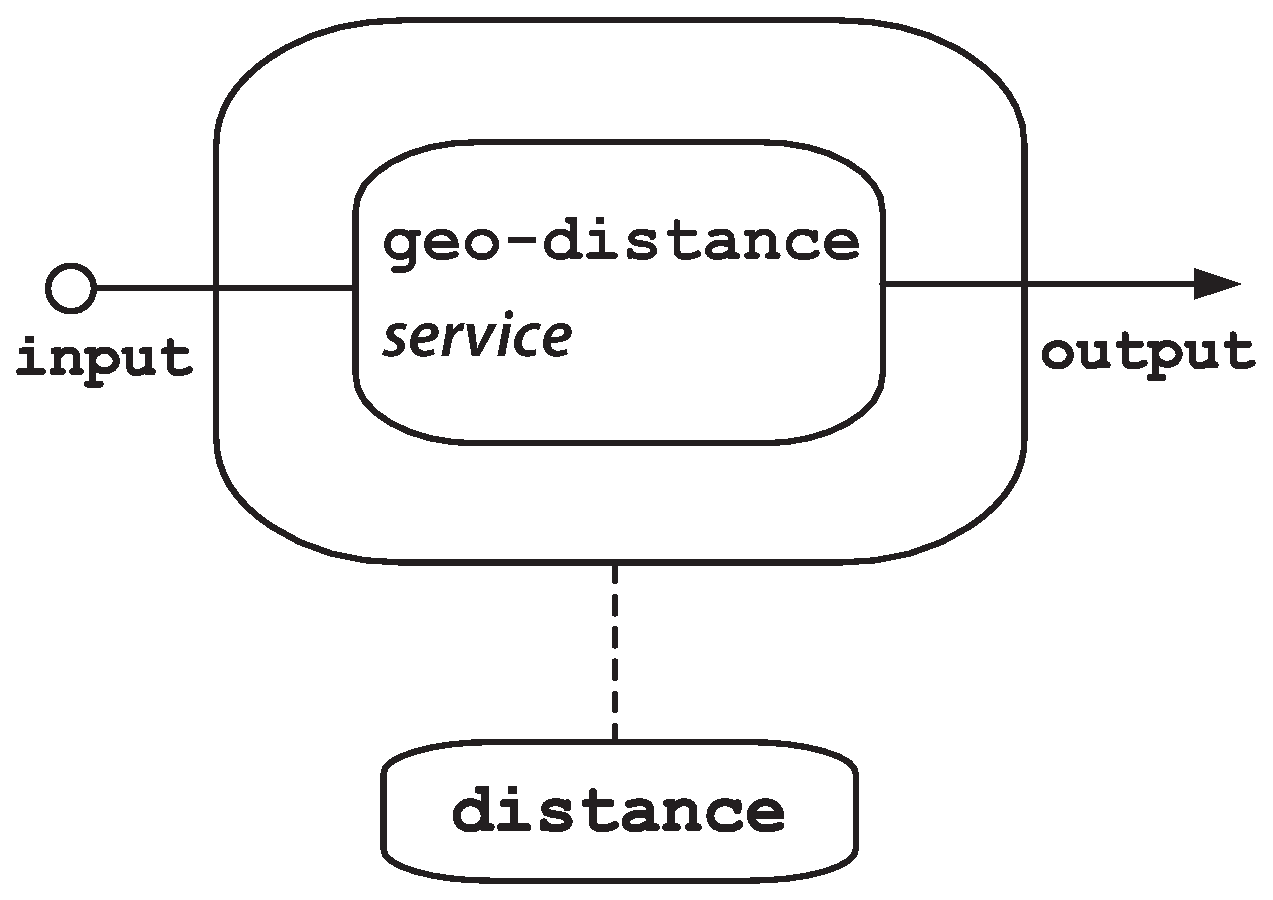
\epsfig{file=Images/Simple.eps, scale=0.2}\label{fig:simpleService}}
				&
				\subfloat[Composite service]{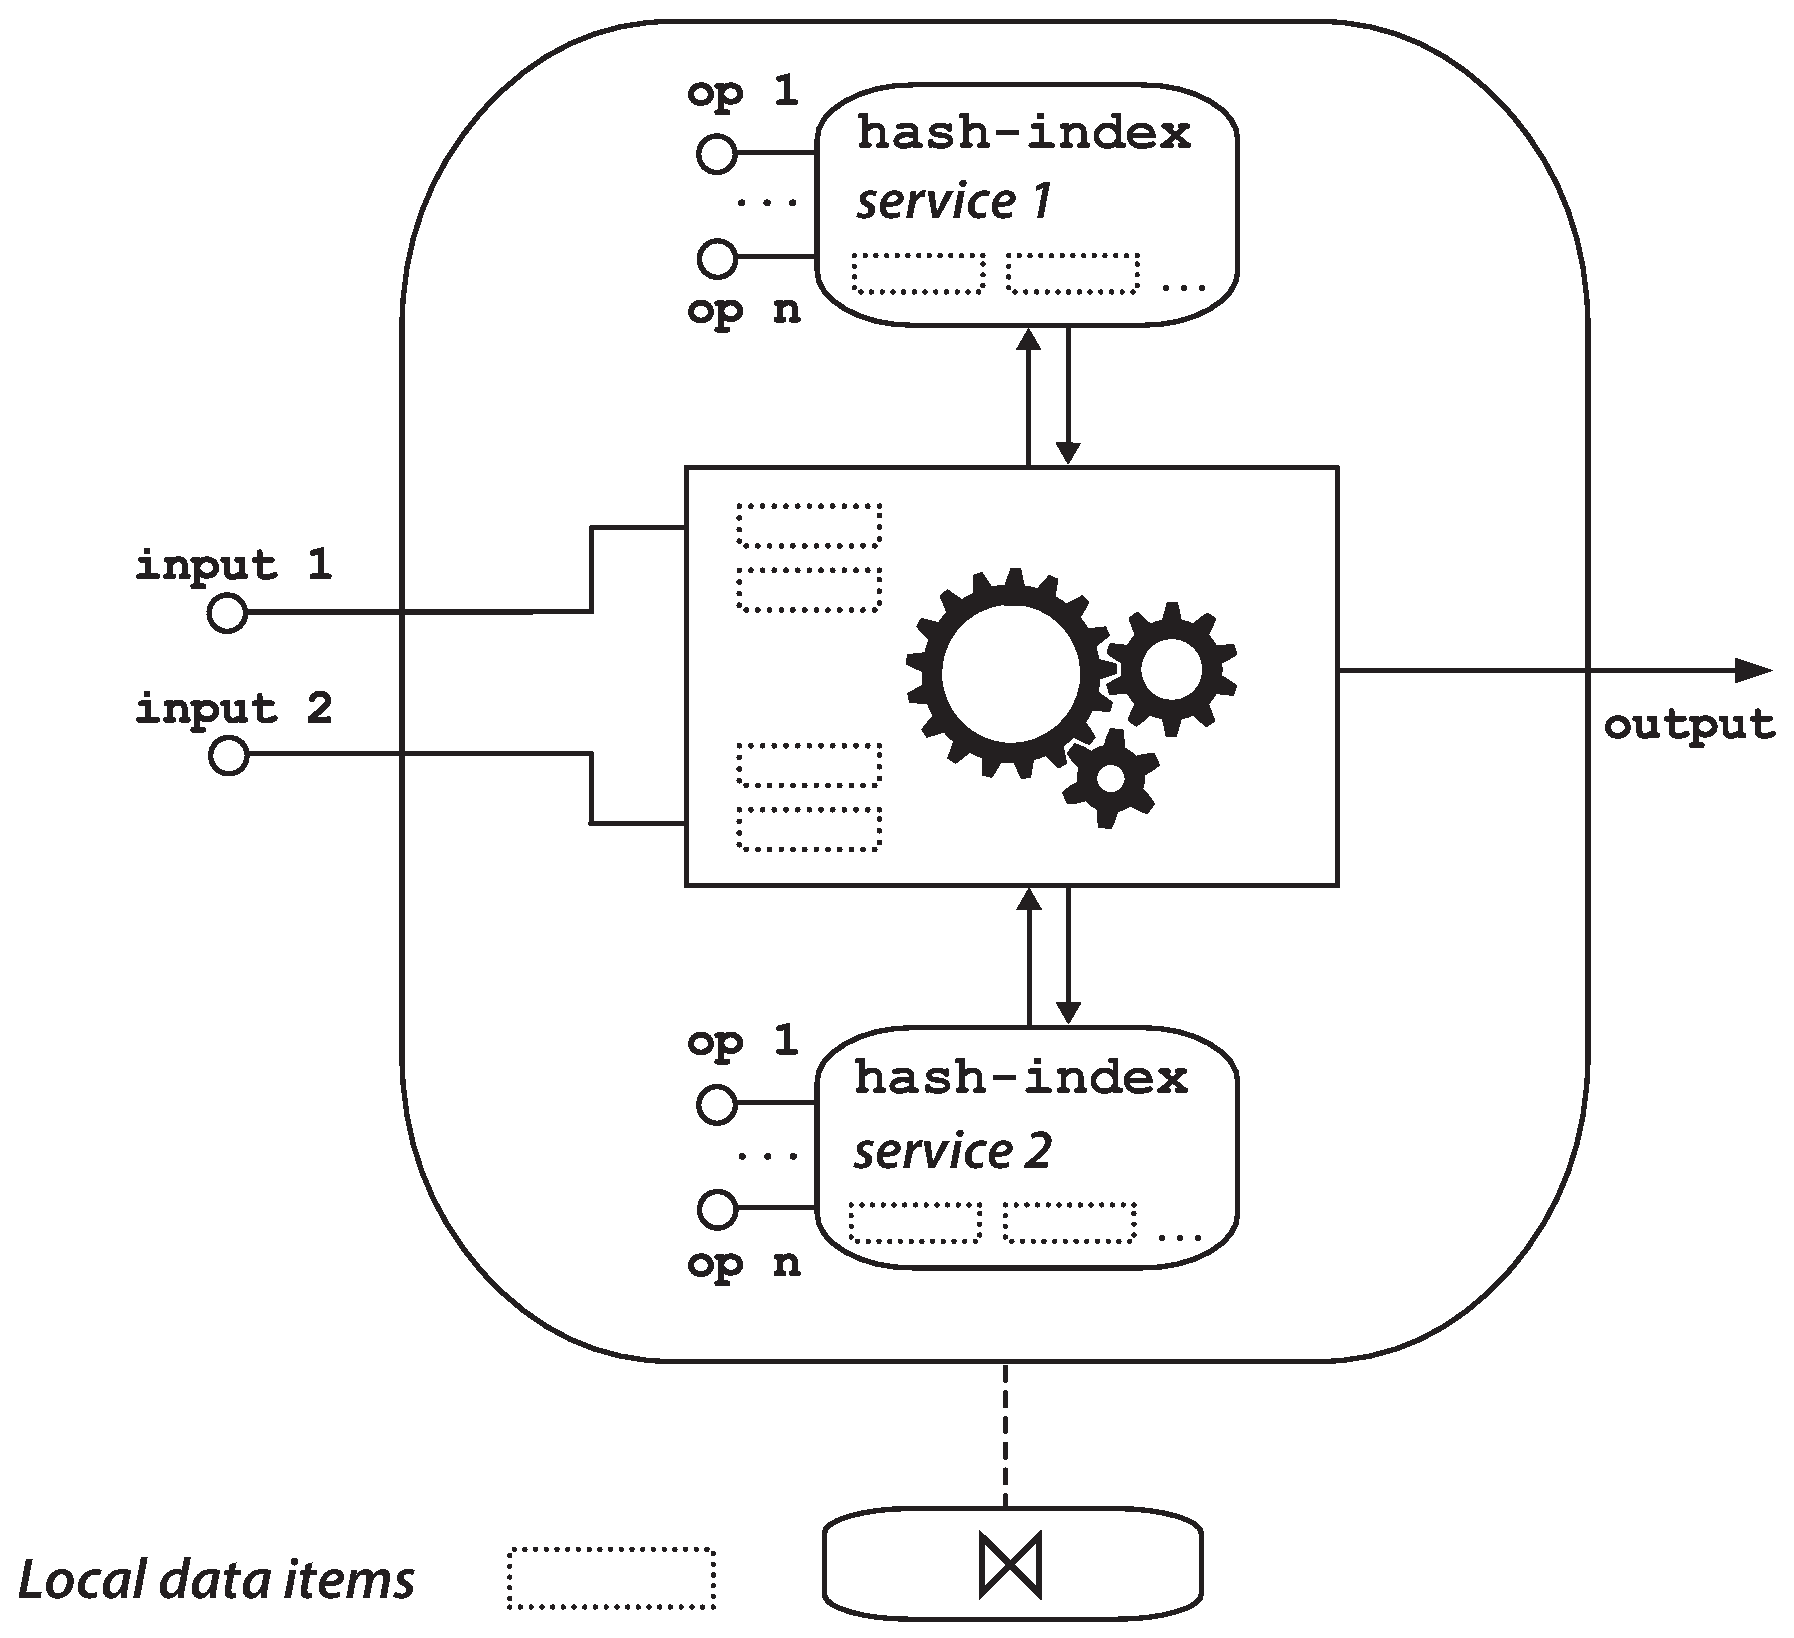
\epsfig{file=Images/Composite.eps, scale=0.2}\label{fig:compositeService}}			
		\end{tabular}
		\caption{Computation services}
		\label{fig:computationServices}
\end{figure*}

\lstdefinelanguage{AbStM}[]{Pascal}{
   morekeywords={seq, endseq, iterate, skip},
}
		
\lstset{language=AbStM,showstringspaces=false}
\begin{lstlisting}[caption={ASM specification for the time-based window},label=TimeWindowListing]
if( ctl_state = 'active')
  seq
     inTuple := readTuple()
     if(inTuple = nil)
        skip
     else
        seq
           oldTuple := cq.peekFirst()
           iterate(oldTuple != nil)
              if(oldTuple.ts + range < inTuple.ts)
                 seq
                    oldTuple.sign := -1
                    oldTuple.ts := oldTuple.ts + range
                    output(oldTuple)
                    cq.removeFirst()
                    oldTuple := cq.peekFirst()
                 endseq
           pq.enqueue(inTuple)
           output(inTuple)
        endseq
  endseq
\end{lstlisting}



		










